

\subsection{Determinism: Type Partitioning}

{  %% chapter slide
%  \setbeamercolor{background canvas}{bg=sectioncolor}
\begin{frame}{\Challenge{4} A Sufficient Type Partitioning}{MDTD: Maximal Disjoint Type Decomposition}
  \only<1>{Given overlapping (super)types $A_1\ldots A_n$ in an RTE}%
  \only<2>{Construct (sub) types $\typevar_1\ldots \typevar_m$}%
  \only<3>{Which are disjoint \Emph{by construction}, even if subtype relation is unknown.}%
  \only<4>{Assures that $\deriv{\typevar}{r}$ is computable.}%
  \only<5>{But transitions may be \Emph{indeterminate} and \Emph{unsatisfiable}.}%
  \begin{columns}
    \begin{column}{0.5\textwidth}
      \only<1,2>{\scalebox{0.98}{\begin{pgfpicture}{0cm}{0cm}{10cm}{6cm} % LL=0,0  UR=10,6
  \pgfcircle[stroke]{\pgfxy(3.5,3)}{3.0cm}   % A   A1
  \pgfputat{\pgfxy(3.5,5.7)}{\pgfbox[center,center]{$A_{1}$}}
  \pgfcircle[stroke]{\pgfxy(2,4)}{1.0cm}   % B    A2
  \pgfputat{\pgfxy(1.5,4.5)}{\pgfbox[center,center]{$A_{2}$}}
  \pgfcircle[stroke]{\pgfxy(3,4.2)}{1.0cm}   % C   A3
  \pgfputat{\pgfxy(3.5,4.6)}{\pgfbox[center,center]{$A_{3}$}}
  \pgfcircle[stroke]{\pgfxy(2.5,2.3)}{1.7cm}   % D A4
  \pgfputat{\pgfxy(1.2,2.7)}{\pgfbox[center,center]{$A_{4}$}}
  \pgfcircle[stroke]{\pgfxy(3.1,1.4)}{0.5cm}   % E   A5
  \pgfputat{\pgfxy(3.2,1.6)}{\pgfbox[center,center]{$A_{5}$}}
  \pgfcircle[stroke]{\pgfxy(5.5,2.0)}{0.5cm}   % F   A6
  \pgfputat{\pgfxy(5.5,2.25)}{\pgfbox[center,center]{$A_{6}$}}
  \pgfcircle[stroke]{\pgfxy(6.7,1.3)}{0.5cm}   % G   A7
  \pgfputat{\pgfxy(6.7,1.5)}{\pgfbox[center,center]{$A_{7}$}}
  \pgfcircle[stroke]{\pgfxy(3.4,1.1)}{1.0cm}   % H   A8
  \pgfputat{\pgfxy(4.0,0.8)}{\pgfbox[center,center]{$A_{8}$}}
\end{pgfpicture}
}}%
      \only<3->{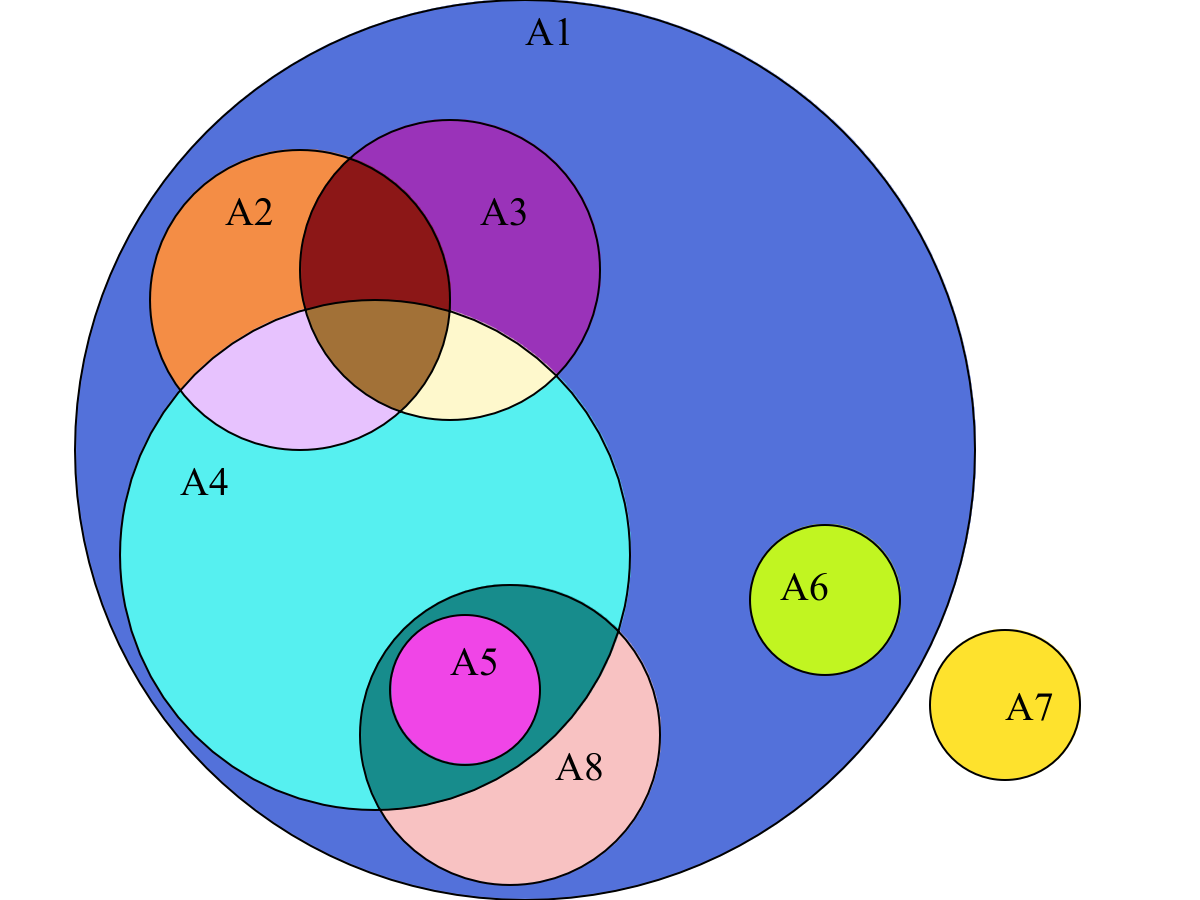
\includegraphics[scale=0.18]{venn-x1-x13.png}}%
    \end{column}%
    \begin{column}{0.5\textwidth}
      \only<2->{\scalebox{0.98}{    \begin{pgfpicture}{0cm}{0cm}{10cm}{6cm} % LL=0,0  UR=10,6
      \pgfcircle[stroke]{\pgfxy(3.5,3)}{3.0cm}   % A   A1
      \pgfputat{\pgfxy(5.5,3.7)}{\pgfbox[center,center]{$\typevar_{1}$}}
      \pgfcircle[stroke]{\pgfxy(2,4)}{1.0cm}   % B    A2
      \pgfputat{\pgfxy(1.7,4.2)}{\pgfbox[center,center]{$\typevar_{2}$}}
      \pgfcircle[stroke]{\pgfxy(3,4.2)}{1.0cm}   % C   A3
      \pgfputat{\pgfxy(2.5,4.4)}{\pgfbox[center,center]{$\typevar_{13}$}}
      \pgfputat{\pgfxy(3.5,4.1)}{\pgfbox[center,center]{$\typevar_{3}$}}
      \pgfputat{\pgfxy(2.5,3.7)}{\pgfbox[center,center]{$\typevar_{11}$}}
      \pgfputat{\pgfxy(2.0,3.4)}{\pgfbox[center,center]{$\typevar_{10}$}}
      \pgfputat{\pgfxy(3.2,3.5)}{\pgfbox[center,center]{$\typevar_{12}$}}
      \pgfcircle[stroke]{\pgfxy(2.5,2.3)}{1.7cm}   % D A4
      \pgfputat{\pgfxy(1.8,1.8)}{\pgfbox[center,center]{$\typevar_{4}$}}
      \pgfcircle[stroke]{\pgfxy(3.1,1.4)}{0.5cm}   % E   A5
      \pgfputat{\pgfxy(3.0,1.3)}{\pgfbox[center,center]{$\typevar_{5}$}}
      \pgfcircle[stroke]{\pgfxy(5.5,2.0)}{0.5cm}   % F   A6
      \pgfputat{\pgfxy(5.5,1.9)}{\pgfbox[center,center]{$\typevar_{6}$}}
      \pgfcircle[stroke]{\pgfxy(6.7,1.3)}{0.5cm}   % G   A7
      \pgfputat{\pgfxy(6.7,1.4)}{\pgfbox[center,center]{$\typevar_{7}$}}
      \pgfcircle[stroke]{\pgfxy(3.4,1.1)}{1.0cm}   % H   A8
      \pgfputat{\pgfxy(3.2,0.45)}{\pgfbox[center,center]{$\typevar_{8}$}}
      \pgfputat{\pgfxy(3.7,1.8)}{\pgfbox[center,center]{$\typevar_{9}$}}
    \end{pgfpicture}
}}%
    \end{column}%
  \end{columns}%
\end{frame}


%% \begin{frame}{Are there dire Consequences?}

%%   \begin{itemize}
%%   \item   $\{\typevar_1, \typevar_2, \ldots, \typevar_{10}\}$ mutually disjoint by construction.
%%   \item   However, some $\typevar_i$ may be unknowingly vacuous.
%%   \item   Nevertheles $\emptyset$ is disjoint with every set, including itself.
%%   \item   Thus transitions may be \Emph{indeterminate/unsatisfiable}.
%%   \item   What is the consequence transitions which are  \Emph{indeterminate} and \Emph{unsatisfiable}?
%%   \end{itemize}
%% \end{frame}

\begin{frame}{DFA with indeterminate transitions: $(int \cdot str^{*} \cdot even)^{*}$}
  \begin{columns}
    \begin{column}{0.5\textwidth}
      \begin{align*}
        p_0 &= (int \cdot str^{*} \cdot even)^{*}\\
        p_1 &= \emptyset\\
        p_2 &= \tystring^{*} \cdot \tyeven \cdot (\tyint \cdot \tystring^{*} \cdot \tyeven)^{*}\\
        p_3 &= \tystring^{*}\!\!\cdot\! \tyeven\!\cdot\! (\tyint\! \cdot\! \tystring^{*}\!\!\cdot\! \tyeven)^{*}\! \reor (\tyint\! \cdot\! \tystring^{*}\!\!\cdot\!\! \tyeven)^{*}
      \end{align*}



      \includegraphics[width=0.9\textwidth,trim={1.4cm 1.2cm 1.4cm 0.8cm},clip=true]{reclojure-2025-sink-example-2}
    \end{column}
    \begin{column}{0.5\textwidth}
      \begin{align*}
        t_1 &= \Sigma\\
        t_2 &= int  \\
        t_3 &= \compl{int}\\
        t_4 &= \textcolor{red}{str \cap even}\\
        t_5 &= \compl{str} \cap even\\
        t_6 &= str \cap \compl{even}\\
        t_7 &= (int \cap \compl{even}) \cup (str \cap \compl{even})\\
        t_8 &= \textcolor{red}{\compl{int} \cap \compl{str} \cap even}\\
        t_9 &=(int \cap even) \cup (str \cap even)\\
        t_{10} &=\compl{str} \cap \compl{even}\\
        t_{11} &=\compl{int} \cap \compl{str} \cap \compl{even}
      \end{align*}
    \end{column}
  \end{columns}
\end{frame}


